\documentclass[conference]{IEEEtran}
\IEEEoverridecommandlockouts
% The preceding line is only needed to identify funding in the first footnote. If that is unneeded, please comment it out.
\usepackage{cite}
\usepackage{amsmath,amssymb,amsfonts}
\usepackage{algorithmic}
\usepackage{graphicx}
\usepackage{textcomp}
\usepackage{xspace}
\usepackage{amsfonts}
\usepackage{algorithm2e}
\usepackage{url}
\usepackage[table,xcdraw]{xcolor}
%\usepackage{soul}

\def\BibTeX{{\rm B\kern-.05em{\sc i\kern-.025em b}\kern-.08em
    T\kern-.1667em\lower.7ex\hbox{E}\kern-.125emX}}
    
\def\system{\texttt{2PLA}\xspace}
\def\dataset{\texttt{ULCER\_SET}\xspace}

\begin{document}

\title{A Two-Phase Learning Approach for the Segmentation of Dermatological Wounds*\\
\thanks{*This work was supported by FAPERJ (G. E-26/203.215/2016 and G. E-11/2018 Sediadas) and FAPESP (G. 2016/17078-0).
Corresponding authors: \textit{\{wellingtons, marcosbedo\}@id.uff.br}.}
}

%\author{\\% <-this % stops a space
%\address{}
%\thanks{$^{2}$P. M. Azevedo-Marques and A. Traina are with University of S\~{a}o Paulo.}
%\thanks{$^{3}$A. Jorge is with S\~{a}o Carlos Federal University.}
%\thanks{$^{4}$L. Santos is with Federal Institute of North of Minas Gerais.}
%\thanks{$^{5}$D. Oliveira is with IC/Fluminense Federal University - Brazil.}
%}

\author{\IEEEauthorblockN{Wellington S. Silva$^{\star}$, Daniel L. Jasbick$^{\star,\dagger}$, Rodrigo E. Wilson$^{\star}$, Paulo M. Azevedo-Marques$^{\bullet}$,\\ Agma J. M. Traina$^{\mp}$, Lucio F. D. Santos$^{\diamond}$, Ana E. S. Jorge$^{\ddagger}$, Daniel de Oliveira$^{\dagger}$, and Marcos V. N. Bedo$^{\star}$}
\IEEEauthorblockA{
$^{\star}$Fluminense Northwest Institute, Fluminense Federal University, Brazil\\
$^{\dagger}$Institute of Computing, Fluminense Federal University, Brazil\\
$^{\bullet}$Ribeir\~{a}o Preto Medical School, University of S\~{a}o Paulo, Brazil\\
$^{\mp}$Department of Computer Science, University of S\~{a}o Paulo, Brazil\\
$^{\diamond}$Federal Institute of North of Minas Gerais -- Montes Claros, Brazil\\
$^{\ddagger}$Department of Physical Therapy, Federal University of S\~{a}o Carlos, Brazil 
}}


\maketitle

\begin{abstract}
Tissue segmentation in photographs of lower limb chronic ulcers is a non-intrusive approach that supports dermatological analyses.
This paper presents \system, a method that combines supervised and unsupervised learning strategies for enhancing the segmentation of dermatological wounds.
Given an ulcer photo captured according to a fixed protocol, \system first phase performs a pixelwise classification of points of interest, whereas pre-processing filters are employed for the smoothing of image noise.
The cleaned image is further sent to the \system divide-and-conquer second phase.
It builds upon SLIC superpixel construction algorithm for dividing the lower limb into regions of interest with well-defined borders, and clusters the superpixels by taking advantage of the similarity-based DBSCAN algorithm.
We set up the phases of our method by using a real annotated set of dermatological wounds, and empirical evaluations on representative samples up to $100{,}000$ points showed a compact Multi-Layer Perceptron with Levenberg--Marquardt training algorithm (Cohen-Kappa = $.971$, Sensitivity = $.98$, and Specificity = $.98$) outperformed other classifiers as \system first phase.
Additionally, experimental trials on DBSCAN with five distance functions ($L_1$, $L_2$, $L_\infty$, Canberra, and BrayCurtis) indicated $L_1$ function provided fewer groups in comparison to the competitors, and the number of clusters was an exponential decay to the similarity ratio.
Accordingly, we used the elbow criterion for finding the $L_1$-based DBSCAN threshold as \system second phase parameterization.
We evaluated the fine-tuned setting of our method over a labeled set of ulcer images, and wounded tissues were segmented within a $.05$ Mean Absolute Error ratio.
These results illustrate the impact of learning parameters on \system as well as the method efficacy for wound segmentation.

\end{abstract}

\begin{IEEEkeywords}
Wound images, Superpixels, MLP, DBSCAN
\end{IEEEkeywords}

\section{Introduction}

Photographs of ulcers in lower limbs have the potential for supporting dermatologists analyses, as they include valuable information regarding the wounded area~\cite{Bates2016} and tissue characterization~\cite{Blanco2016,Todd2018}.
Image obtaining is a non-intrusive process, \textit{e.g.}, smartphone-based image recording~\cite{Deserno2018,Goyal2018}, while digital photo management can be carried out by non-complex engines in comparison to radiological systems~\cite{Gillies2015}.
Such advantages favor the exponential increase in the number of annotated photos digitally stored, which gives room for the design of new Computer-Aided Diagnosis (CAD) tools~\cite{Chino2018,Deserno2018}.
In contrast to pattern recognition tasks that aims at classifying and reporting skin abnormalities~\cite{Zahia2018}, the analysis of chronic ulcers are rather related to the \textit{segmentation} of wounded tissues so that they can be further integrated with patient data, previous diagnoses, or even radiomics systems~\cite{Gillies2015}.

Challenges regarding the design of segmentation methods for chronic ulcers in lower limbs consist of \textit{(i)}~characterizing particular types of tissues and 
\textit{(ii)}~quantifying tissue areas within and around wounded regions~\cite{Pereyra2014,Todd2018}.
Typically, CAD methods are based on either \textit{supervised} or \textit{unsupervised} learning paradigms.
Supervised approaches heavily rely on classification algorithms for the separation of  healthy skin pixels from those \textit{within} the ulcered region.
Godeiro et al.~\cite{Godeiro2018} use a color space reduction for the extraction of wounded regions according to their most dominant tissues at $94\%$ Dice Coefficient ratio.
Mukherjee et al.~\cite{Mukherjee2014} apply low-level color extractors and Support-Vector Machines for the labeling of chronic wounds into five classes at $87.61\%$ hit ratio.
Blanco et al.~\cite{Blanco2016} and Chino et al.~\cite{Chino2018} use the same set of five labels, but apply a divide-and-conquer strategy in which wounds are segmented with the support of superpixel construction methods~\cite{Achanta2012,Barbieri2015}.
Such methods divide an image into regions of interest with well-defined borders that are further extracted by feature engineering methods, as MPEG-7 descriptors~\cite{Blanco2016} or Bag-of-Signatures~\cite{Chino2018}. 
Extracted features are labeled by RandomForest in up to $89.87\%$ accuracy.

Deep-learning models combine both image extraction and data classification into a single package, which removes the need for feature engineering methods.
Goyal et al.~\cite{Goyal2018} use a deep network for the segmentation of diabetic ulcers into three groups at $92.5\%$ accuracy ratio, while Zahia et al.~\cite{Zahia2018} define a convolutional network for segmenting pressure ulcers at $91.3\%$ Dice Coefficient ratio.
The main drawback with \textit{supervised-only} approaches is they do not differ all tissue combinations within and around the wound by assuming a fixed and discrete set of labels (\textit{e.g.}, ``granulation'' or ``slough'') for splitting the image into ulcer and skin.

On the other hand, unsupervised methods describe chronic wounds by clustering similar regions into single tissue pieces, whereas ulcer borders are kept \textit{around} the wounded tissues~\cite{Dhane2017,Bates2016}.
Maity et al.~\cite{Maity2018} surveyed Region Growing, $k$-Means, Fuzzy $C$-means, and Gaussian Mixture Model algorithms for the analysis of venous ulcers, and results indicated Gaussian Mixture Model segmented chronic wounds at $95.91\%$ Sensitivity ratio.
Likewise, Dhane et al~\cite{Dhane2017} described a new fuzzy method for ulcer segmentation with up to $91.5\%$ accuracy ratio. 
Clustering approaches provide the basis for measuring the size, volume, and stage of the wounds, which enhances final diagnoses~\cite{Bates2016,Todd2018}.
However, as computational complexity of \textit{unsupervised-only} methods is gradually affected by the number of regions of interest, clustering routines can become time and power consuming, and, consequently, unsuitable for personal computers and battery-bounded devices~\cite{Deserno2018}. 

Aiming at surpassing those drawbacks, we propose a new approach that combines the best of supervised and unsupervised paradigms.
Our method, named \system (\textit{\textbf{T}wo-\textbf{P}hase \textbf{L}earning \textbf{A}pproach}), is a two-phase approach that removes points of no-interest (\textit{e.g.}, background area) for reducing the number of candidate regions to be clustered into different tissue pieces.
Given a wound photo recorded by a fixed protocol, \system first phase performs a pixelwise classification of potential points of interest, while pre-processing filters smooth lower limb borders.
\system second phase processes the cleaned data by using a divide-and-conquer strategy. 
It builds upon SLIC~\cite{Achanta2012} superpixel construction algorithm for dividing the lower limb into regions of interest with well-defined borders, and clusters the superpixels by taking advantage of the similarity-based DBSCAN algorithm~\cite{Kriegel2017}.

Since both \system phases are parametric, we discuss the tuning of pixel classification and superpixel clustering algorithms by using a real and annotated set of dermatological wounds.
Empirical evaluations on representative samples up to $100{,}000$ points showed a compact Multi-Layer Perceptron with Levenberg--Marquardt training method outperformed other classifiers as \system first phase.
We also evaluated DBSCAN performance with regards to five distance functions ($L_1$, $L_2$, $L_\infty$, Canberra, and BrayCurtis) and results indicated $L_1$ function generates fewer groups in comparison to the competitors, and the number of clusters is an exponential decay to the similarity ratio.
Accordingly, we used the elbow criterion~\cite{Jolliffe2011} as the $L_1$-based DBSCAN threshold for tuning \system second phase.
Finally, we performed an experiment with fine-tuned \system on real images and results showed tissues were segmented at a low error ratio.
In summary, the main contributions of this study are as follows:

\begin{itemize}
\item \underline{Wound segmentation}: We designed a two-phase approach (\system) that combines supervised and unsupervised learning for the segmentation of chronic wounds.

\item \underline{\system tuning}: We tuned our approach through empirical evaluations on a real set of ulcers.
Results indicated MLP, $L_1$ and the elbow criterion as suitable \system parameters.
\end{itemize}

The remainder of this paper is structured as follows. 
Section~2 introduces the basic concepts of the paper and the main related work. 
The proposed method is described in Section~3. 
Section~4 presents the experiments and discusses the results. 
Finally, Section~5 presents the conclusions and future work.


\section{Background and Related Work}\label{sec:background}

Visual ulcer assessment is carried out by clinicians through the evaluation of wounded tissues and their adjacent skin.
Such an evaluation is made upon ulcer size, edges, wounded tissue types and their area, surrounding skin color, peripheral edema, and epithelialization~\cite{Todd2018}.
Ulcer measurement is a key metric for keeping track of wound healing ratio and progress, while the separation of distinct tissue types and the quantification of their areas constitute major beacons for assessing wound health status.
Commonly, there is a non-uniform \textit{overlapping} of tissues within the ulcerated lower limb region depending on its healing stage.
For instance, granulation tissues originated in the proliferative phase can appear mixed with fibrin, \textit{i.e.}, non-viable tissues, or even with necrosis, whenever the number of bacteria is not properly under control~\cite{Pereyra2014}.
Analogously, surrounding wound skin provides crucial information about therapeutic intervention and treatments.
For example, adjacent skin may include scar formation, hyperkeratosis, pathogenic inflammatory signs, and hyper\-pigmentation in cases of chronic and venous ulceration~\cite{Todd2018}.

Therefore, the design of a CAD method for ulcer segmentation depends on distinguishing wounded tissues \textit{within} and \textit{around} ulcered areas.
Classification-only approaches represent skin content as feature vectors and label them according to biased functions, which are previously induced by a training set of examples.
Feature vectors are extracted from either feature engineering methods~\cite{Sonka2014}, or auto encoders of convolutional neural networks~\cite{Aggarwal2018}, whereas classifier methods are derived from several paradigms, as Na\"{i}ve-Bayes (NB), Bayes-Net (BN), Instance-based Learning (IbL), Multi-Layer Perceptron with Levenberg--Marquardt (MLP-LM) or Rprop training algorithms (LMP-RP), Decision-Tree (DT), and RandomForest (RF)~\cite{Aggarwal2015}.
The proposals in~\cite{Kavitha2017,Blanco2016,Chino2018} employ feature engineering methods for the classification of a dermatological ulcer according to the type of the majority of wounded tissues.
Analogously, the approaches in~\cite{Deserno2018,Godeiro2018,Zahia2018} apply deep-learning methods for extracting and classifying five types of wounds according to their most dominant tissues.
The main drawback with such approaches is they disregard \textit{mixed} wound types, as in evolving borders or epithelialization where the number of tissue combinations is virtually unlimited.

Clustering approaches are alternatives to supervised methods, as they group both border and interior tissues according to their similarity.
For instance, the studies~\cite{Maity2018,Dhane2017} apply Gaussian Mixture Models, Hard and Fuzzy clustering for the segmentation of wounded and border tissues.
Although such strategies provide a more comprehensive ulcer segmentation and support the pixelwise measurement of wounded areas, their running time is affected by the number of regions of interest, and, therefore, their processing may be unsuitable for local and power-limited mobile devices~\cite{Deserno2018}.

Our premise is combining supervised and unsupervised learning improves current state-of-the-art wound segmentation since the number of regions of interest to be clustered can be reduced through a classification-first phase.\\

\noindent 
\textbf{Notation.}
An \textit{image} $I$ is a structured set of $n$ pixels, \textit{i.e.}, $I = \{P_{i} ~|~ 0 \leq i < n \}$.
A pixel $P_i$ is a tuple $P_{i} =  \langle r_{i}, g_{i}, b_{i} \rangle$, where $r_{i}, g_{i}$, and $b_{i}$ are the pixel coordinates in the $RGB$ color space~\cite{Sonka2014}.
A \textit{superpixel} $S$ corresponds to a structured subset $S \subseteq I$ defined as $S = \{P_{j} ~|~ 0 \leq j < m \}$, where $m ~(m \leq n)$ is the number of pixels inside superpixel $S$. 
The superpixel average value $\bar{P_S}$ is a tuple $\bar{P_S} = \langle \mu(r), \mu(g), \mu(b)\rangle$, in which $\mu(k) = \sum_{j = 0}^{m-1} k_j/m$.
The set of images is denoted by $\mathcal{I}$, and the set of superpixels is denoted by $\mathcal{S}$.\\

\noindent 
\textbf{Color space transformation.} 
The $Lab$ color space transformation is a function $\varepsilon: RGB \rightarrow Lab$ that maps an $RGB$ coordinate into a point of the $Lab$ space.
Given a pixel $P_i$, $\varepsilon$ calculates the mapped $Lab$ point as in Equation~\ref{eq:rgb2Lab}.
\begin{equation}\label{eq:rgb2Lab}
\begin{split}
L = 116*f\left(\frac{y_i}{100}\right) - 16,\\
a = 500*f\left(\frac{x_i}{95.047} - \frac{y_i}{100}\right), \\
b = 200*f\left(\frac{y_i}{100} - \frac{z_i}{108.883}\right),\\
f(k) =
\begin{cases}
    \sqrt[3]{k},     & \text{if } k > (6/29)^3 \\
    \frac{k}{3*(6/29)^2} + \frac{4}{29}\,   & \text{otherwise}
\end{cases},\\
\begin{bmatrix}
    x_i\\
    y_i\\
    z_i
\end{bmatrix}
=
\begin{bmatrix}
    .4124 & .3576 & .1805 \\
    .2126 & .7152 & .0722 \\
    .0193 & .1192 & .9505
\end{bmatrix}
\cdot
\begin{bmatrix}
    r_i\\
    g_i\\
    b_i
\end{bmatrix}
\end{split}
\end{equation}\\

\noindent
\textbf{Superpixel segmentation.}
Pixels within a superpixel are automatically selected from an image according to a \textit{superpixel construction algorithm}.
Such algorithms are functions $G(I, K_p) = \{S_j ~|~ 0 \leq j < K_p\}$ that take one image $I$ and generate $K_p$ disjoint and non-empty superpixels $S_j, ~S_j \subset I$.
Comparative surveys for state-of-the-art superpixel algorithms~\cite{Achanta2012,Barbieri2015} indicate SLIC method provides good adherence to image boundaries, and it is the most efficient strategy for superpixel generation.\\

\noindent
\textbf{Classifier.}
A classifier $\phi$ is a function $\phi: \{\mathcal{P}, T\} \rightarrow L$, where $L$ is a discrete and disjoint set of labels, $\mathcal{P}$ is the pixel domain, and $T$ is a training set that conditions the behavior of $\phi$~\cite{Aggarwal2015}.
In the context of this study, $T$ summarizes a finite and non-empty set of labeled pixels, \textit{i.e.}, $T = \{\langle P_i, l_j\rangle~| L = \cup_j l_j\}$, and the classifier \textit{learning algorithm} is a biased method that induces the behavior of $\phi$ from $T$ to predict a label $l \in L$ for any pixel $P_j \in \mathcal{P} \subseteq \mathcal{I}$.
Examples of classifiers for wounded tissue classification include DT, NB, BN, DS, MLP-LM, MLP-RP, IbL, and RF methods~\cite{Blanco2016,Chino2018,Veredas2010,Kavitha2017}.\\


\noindent
\textbf{Partitional Clustering.} 
A crisp clustering method is a function $\theta$ that partitions data entries into a set of disjoint clusters.
Given a set of superpixels $\mathcal{S}$ and a set of groups $\mathcal{C}$, clustering method $\theta: \mathcal{S} \rightarrow \mathcal{C}$ assigns each superpixel $S \in \mathcal{S}$ to only one cluster $C \in \mathcal{C}$ so that $\cup_{C_i \in \mathcal{C}} C_i = \mathcal{S}$ and $\cap_{C_i \in \mathcal{C}} C_i = \emptyset$.\\


\noindent
\textbf{Similarity metric.} 
A similarity metric is a distance function $\delta: \mathbb{M} \times \mathbb{M} \rightarrow \mathbb{R}_{+}$ that measures the distance bewteem two points in $\mathbb{M}$, \textit{e.g.}, $Lab$ coordinates.
Semantically, the farther the points, the higher their dissimilarity.
For any $m_1, m_2, m_3 \in \mathbb{M}$, $\delta$ satisfy the following axioms: 
\textit{(i)}~symmetry; 
\textit{(ii)}~non-negativity; and 
\textit{(iii)}~triangle inequality.
Therefore, branch-and-bound searching routines take advantage of such axioms for speeding up pairwise comparisons~\cite{Hetland2009}.




\section{Material and Method}

\begin{figure*}[!htb]
\centering
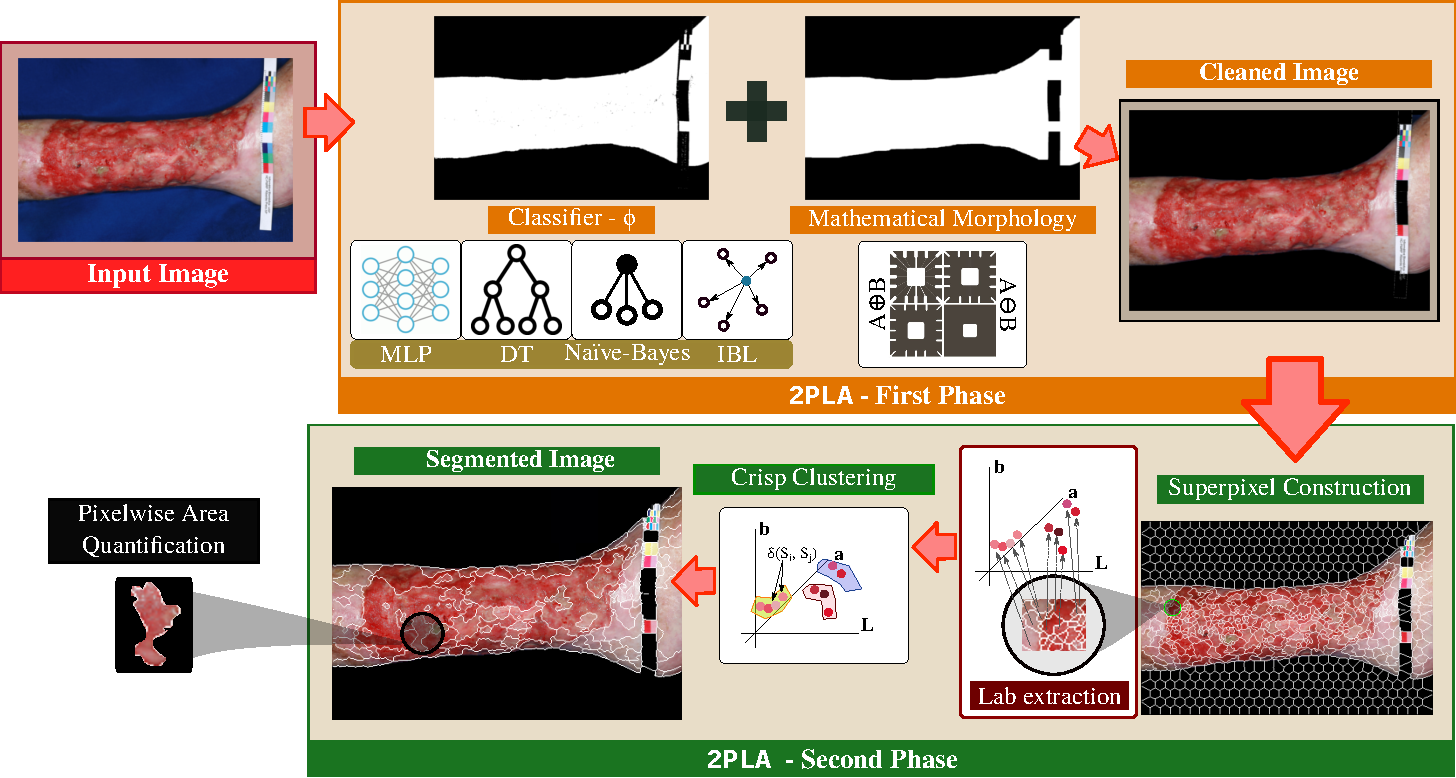
\includegraphics[scale=.66]{figs/pipeline2.pdf}
\caption{Overall \system pipeline.
\system first phase removes background points through pixelwise classification and mathematical morphology.
Cleaned images are divided into superpixels further represented in the $Lab$ color space.
\system second phase applies a crisp cluster approach for grouping similar superpixels, and joint regions can be masked back into the input image. 
Segmented tissues are quantified regarding the number of inner pixels.}
\label{fig:system}
\end{figure*}
This section describes a two-phase method for chronic wound segmentation as well as the ulcer dataset we employed for the tuning and evaluation of our approach.\\

\noindent
\textbf{Data source.} 
We consider data source \dataset~\cite{Pereyra2014} in the design and evaluation of our proposal.
Such an image set includes $217$ photographies of venous and arterial ulcers in lower limbs with varying sizes and distinct healing stages regarding patients with different skin colors, age, and treatments.
Blue and white cloths were used to emphasize the contrast between the background and the patients' skin, and photos were taken with the same camera, angle and distance.
Color patches and rulers were also included in the images to facilitate color normalization and area calibration.
We asked experts to provide a manual segmentation of $40$ representative \dataset images to be used as the \textit{ground-truth} in all subsequent evaluations.
As a result, millions of pixels were labeled as ``background'' and ``skin'', while regions of interest were divided into ``border'' and ``interior'' tissues, which include parts of granulation, fibrin, and necrosis.\\


\noindent
\textbf{\system pipeline.} 
Our proposal, named \system, can be seen as a sequential pipeline for chronic wounds segmentation\footnote{\url{github.com/sswellington/2PLA}}.
The main idea is removing background points eases the similarity-based clustering of superpixels with well-defined borders.
Figure~\ref{fig:system} describes \system pipeline according to a sample image from \dataset.
In \system first phase, pixels of class ``skin'' are selected as relevant, whereas ``background'' pixels are dismissed.
Potential misclassifications of pixels at lower limb borders are rectified by the following morphological operators 
\textit{(i)}~median filter, 
\textit{(ii)}~Otsu binarization of skin pixels, and 
\textit{(iii)}~opening.
%The morphological structuring element perimeter is set to $1\%$ of the input image perimeter.
Cleaned images are fed to \system  divide-and-conquer second phase, in which background-free images are divided into superpixels by SLIC construction algorithm, while superpixel average values are extracted into the $Lab$ color space.
Next, DBSCAN is employed for the grouping of extracted points according to their similarity and density.
Clustered superpixels are joint into a single piece of tissue, which is quantified regarding the number of inner pixels.

Algorithm~\ref{alg:1} relies on a set of parameters for the implementation of \system pipeline.
Parameter $K_p$ defines the number of constructed superpixels, and parameter $\phi$ is a trained classifier for the labeling of skin pixels, whereas parameters $\delta$ and $\xi$ are DBSCAN settings that define how the similarity between two superpixels is measured and maximum dissimilarity threshold, respectively.
Accordingly, the tuning of \system depends on setting suitable values for Algorithm~\ref{alg:1} parameters.
\vspace{-7px}

\SetKwFunction{slic}{SLIC}
\SetKwFunction{dbscan}{DBSCAN}
\SetKwFunction{morph}{MATH\_MORPHOLOGY}
\SetKwInOut{Input}{Input}
\SetKwInOut{Output}{Output}
\begin{algorithm}[!htb]
\small
\hrulefill

 \Input{Image $I$, metric $\delta$, similarity threshold $\xi$, number of superpixels $K_p$, and trained classifier $\phi$.}
 \Output{Segmented tissues within and around the ulcer.}
 \vspace{-4px}
 \hrulefill
 
 $P_a \leftarrow \langle 0, 0, 0\rangle$\;
\tcc{Discards points of no-interest}
\For{$P_i \in I$}{
    \If{$\phi(P_i) \neq$ ``skin''}{
        $P_i \leftarrow P_a$\;
    }
} %For
$I \leftarrow$ \morph{$I$}\;
$\mathcal{S} \leftarrow$ \slic{$I$, $K_p$}\;
\tcc{Discards $S \in \mathcal{S}$ whenever $\varepsilon(\bar{P_S}) = \varepsilon(P_a)$}
$\mathcal{S'} \leftarrow$ \dbscan{$\mathcal{S}, \delta, \xi, P_a$}\;
\Return $\mathcal{S'}$ masked on $I$\;
 \vspace{-4px}
\hrulefill
 \vspace{2px}
\caption{\system implementation.}
\label{alg:1}
\end{algorithm}
\vspace{-12px}




\section{Experiments}

This section reports on \system experiments in an Ubuntu 16.04.4 LTS OS running in $04$ cores of local $i7~3.7$GHz processors with 08 Gb RAM.
Particularly, we evaluated \system in a set of experiments on \dataset for 
\textit{(i)}~tuning \system first phase,
\textit{(ii)}~addressing the gains of pixelwise classification,
\textit{(iii)}~tuning \system second phase, and
\textit{(iv)}~assessing \system quality in tissue segmentation.\\

\noindent
\textbf{Tuning of \system first phase.}
We experimented on $40$ labeled \dataset images for the tuning of \system classification phase.
Image pixels were manually separated into background and skin pixels resulting in more than 100 million points, which were sampled, with stratification by class, into sets of $1 \cdot 10^1, 1 \cdot 10^2, 1 \cdot 10^3, 1 \cdot 10^4$ and $1 \cdot 10^5$ pixels.
Figure~\ref{fig:sample} shows the RGB plots for samples $1 \cdot 10^3, 1 \cdot 10^4$ and $1 \cdot 10^5$, in which points are divided into two separated groups.

\begin{figure}[!htb]
\centering
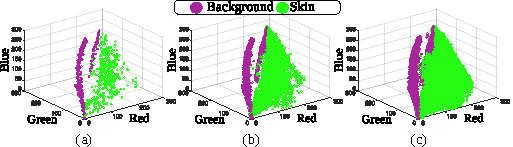
\includegraphics[scale=1.02]{figs/plots.pdf}
\caption{RGB points for samples
(a)~$1 \cdot 10^3$,
(b)~$1 \cdot 10^4$, and
(c)~$1 \cdot 10^5$.}
\label{fig:sample}
\end{figure}

\begin{figure*}[!htb]
\centering
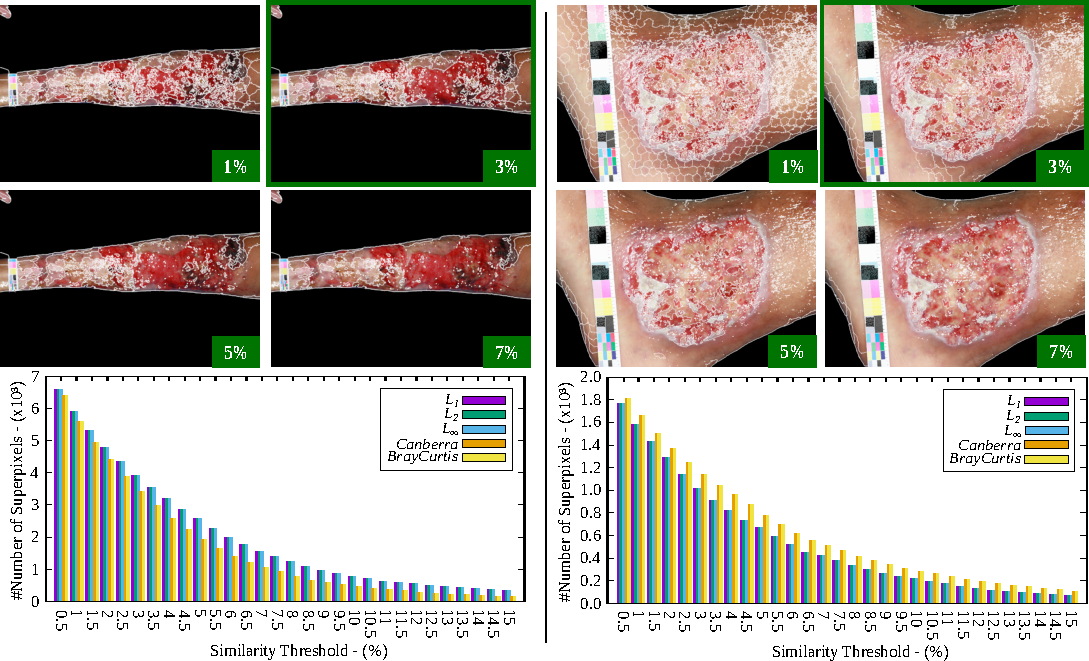
\includegraphics[scale=.84]{figs/res2.pdf}
\vspace{-6px}
\caption{Bar plots for \system second phase tuning, and two wound segmentation examples for increasing $L_1$-based DBSCAN similarity thresholds.}
\label{fig:expto_dbscan}
\end{figure*}

Such a two-class pixel classification problem was addressed through 10-folds cross-validation tests over classifiers previously used in related works, namely Na\"{i}ve-Bayes (NB), Bayes-Net (BN), Instance-based Learning (IbL), Multi-Layer Perceptron with Levenberg--Marquardt (MLP-LM) and Rprop training algorithms (LMP-RP), Decision-Tree (DT), and RandomForest (RF).
Table~\ref{tab:classifiers} shows the scores of Cohen-Kappa Coefficient (CKC) for each classifier and indicates MLP-LM and RF outperformed the competitors in most of the samples (bold column values).
Accordingly, we selected MLP-LM as the \system first phase classifier as it reached the best scores for both weighted ($\bar{\mu}$) and simple ($\mu$) CKC mean.
Although only CKC is reported due to space limitations, MLP-LM also reached the highest ratings for weighted classification metrics Sensitivity ($.98$) and Specificity ($.98$).
\vspace{-10px}

\begin{table}[!htb]
\centering
\caption{Cohen-Kappa Coefficient (CKC) for \system first phase.}
\vspace{-5px}
\label{tab:classifiers}
\begin{tabular}{l|c|c|c|c|c||c|c} \hline \hline
 & 
\multicolumn{7}{c}{ {\cellcolor[HTML]{68CBD0}\textbf{Sample Size}} }    \\ \hline
\cellcolor[HTML]{68CBD0} \textbf{Classifier} & 
\cellcolor[HTML]{68CBD0} \textbf{$10^1$}  & 
\cellcolor[HTML]{68CBD0} \textbf{$10^2$}  & 
\cellcolor[HTML]{68CBD0} \textbf{$10^3$}  & 
\cellcolor[HTML]{68CBD0} \textbf{$10^4$}  & 
\cellcolor[HTML]{68CBD0} \textbf{$10^5$}  &
\cellcolor[HTML]{68CBD0} \textbf{$\bar{\mu}$} &
\cellcolor[HTML]{68CBD0} \textbf{$\mu$}\\ \hline \hline
NB         & .156 & .710 & .793 & .797 & .805  & .804 & .652 \\ \hline
BN         & .038 & .423 & .639 & .722 & .743  & .739 & .513 \\ \hline
%DS         & .025 & .541 & .443 & .408 & .411  & .411 & .365 \\ \hline
IbL        & .675 & .874 & \textbf{.967} & \textbf{.967} & .971 & .970 & .890\\ \hline
\textbf{MLP-LM} & \textbf{.697} & \textbf{.895} & .953 & \textbf{.967} & \textbf{.972} & \textbf{.971} & \textbf{.896} \\ \hline
MLP-RP     & .423 & .829 & .929 & .958 & .968  & .967 & .821 \\ \hline
DT         & .493 & .790 & .922 & \textbf{.967} & .970  & .969 & .828 \\ \hline
%RT         & .217 & .855 & .941 & .964 & .970  & .969 & .789 \\ \hline
RF         & .350 & .854 & .947 & \textbf{.967} & \textbf{.972} & \textbf{.971} & .818\\ \hline \hline
\end{tabular}
\end{table}

\noindent
\textbf{Discarding of superpixels.}
We measured the impact of background removal by calculating the number of regions of interest eliminated from \system second phase after the pixelwise classification.
Figure~\ref{fig:efic} shows the mean and standard deviation for the proportion of discarded regions of interest in a varying number of superpixels ($K_p$) regarding $40$ images.
The higher the discard ratio, the more efficient is \system for eliminating candidate regions.
Consolidated results indicate discarding ratio grew linearly to the number of superpixels and reached up to $48\%$ of dismissed regions for $K_p = 10 \cdot 10^3$.\\

\noindent
\textbf{Tuning of \system second phase.}
We evaluated the impact of two DBSCAN parameters upon $40$ \dataset images with background removed by \system first phase.
In particular, we experimented on five metrics $\delta = L_1$, $L_2$, $L_\infty,$ Canberra, and BrayCurtis and $30$ thresholds ranging from $\xi = 0.5\%$ to $\xi = 15\%$ of maximum dissimilarity in steps of $0.5\%$.
Figure~\ref{fig:expto_dbscan} shows two segmentation examples for DBSCAN and the experimented settings.
Canberra and BrayCurtis presented a wider variance regarding the number of groups by thresholds, while functions $L_1$, $L_2$ and $L_\infty$ exhibited a stable behavior, \textit{i.e.}, lower variances. 
Function $L_1$ also generated fewer clusters in comparison to other metrics for all thresholds, on average.

\begin{figure}[!htb]
\centering
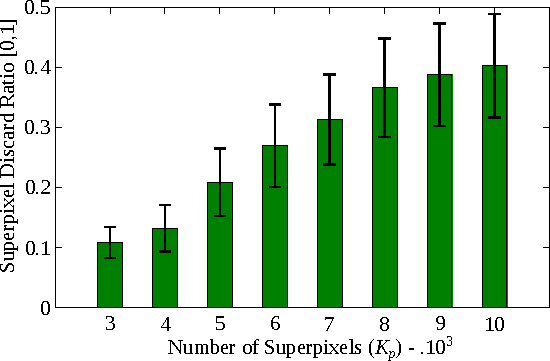
\includegraphics[scale=.68]{figs/efic.pdf}
\vspace{-8px}
\caption{\system first phase superpixel elimination ratio.}
\label{fig:efic}
\end{figure}

Figure~\ref{fig:expto_dbscan} also provides two examples of bar plots regarding the number of groups and the similarity thresholds.
Bar plots of evaluated images resembled an exponential decay function, whose slope is leveling off towards the curve ``elbow''.
Accordingly, we took advantage of such behavior for applying the elbow criterion of Scree-Plot factor analysis~\cite{Jolliffe2011} for the setting of the DBSCAN threshold.
The premise is the curve elbow indicates where the bar plot starts to smooth up so that the cut point can be determined by the first of two consecutive bars whose difference ratio does not exceed a fixed threshold $\Delta, \Delta \leq \frac{bar_i - bar_{i+1}}{bar_i}$.

Hence, we experimented with $\Delta$ ranging from $5\%$ to $20\%$ of the bar difference ratio in steps of $1\%$, and the most frequent cut point regarding the $40$ evaluated images was the similarity threshold $\xi = 3\%$.
Figure~\ref{fig:expto_dbscan} highlights two examples of superpixel clustering (green borders) carried out by DBSCAN with these suitable settings, \textit{i.e.}, distance $\delta = L_1$, and threshold $\xi = 3\%$.\\

\noindent
\textbf{Pixelwise area quantification.} 
In the last experiment, we separated 04 new and diversified \dataset images that were manually segmented by an expert.
Figures~\ref{fig:quantification}(a--b) show one of the selected images and the expert-provided segmentation, while Figures~\ref{fig:quantification}(c--d) illustrate the outputs of \system first and second phase, respectively.
\system segmented pixels were matched to expert segmentation with a Mean Absolute Error (MAE) ratio of $.05$  (variance of $.01$), which indicates a high separation ratio through the divide-and-conquer strategy.

\begin{figure}[!htb]
\centering
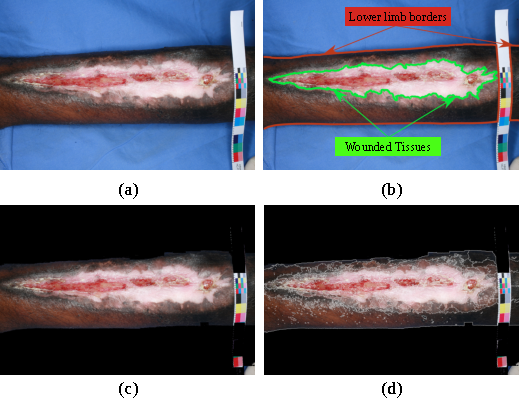
\includegraphics[scale=.96]{figs/quantification1.pdf}
\vspace{-8px}
\caption{(a)~Example of an \dataset image, and
(b)~manual tissue segmentation.
(c)~\system first phase output, and
(d)~\system outcome.}
\label{fig:quantification}
\end{figure}






\section{Conclusions and Future Work}

This study has discussed a two-phase segmentation approach for detaching pieces of tissues within and around dermatological ulcers.
The method, called \system, combines supervised and unsupervised learning for reducing the number of regions of interest and the clustering of visually similar tissues.
Empirical evaluations on a real image set indicated \system effectively separated skin and background pixels at $.971$ CKC, and efficiently reduced the number of superpixels to be clustered in up to $48\%$.
Additionally, experiments showed $L_1$ was the metric that generated fewer groups in comparison to the competitors, and the number of clusters is an exponential decay to the similarity threshold.

Accordingly, \system was fine-tuned with elbow criterion for determining the clustering threshold.
We also compared \system to manual segmentation, and results showed \system quantified the pixelwise area at a $.05$ MAE ratio.
Future works include \system extension for handling superpixel convolutional features as well as the evaluation of hierarchical clustering methods as \system second phase.



\bibliographystyle{plain}
\bibliography{biblio}


%section*{References}

%Please number citations consecutively within brackets \cite{b1}. The 
%sentence punctuation follows the bracket \cite{b2}. Refer simply to the reference 
%number, as in \cite{b3}---do not use ``Ref. \cite{b3}'' or ``reference \cite{b3}'' except at 
%the beginning of a sentence: ``Reference \cite{b3} was the first $\ldots$''

%%Number footnotes separately in superscripts. Place the actual footnote at 
%the bottom of the column in which it was cited. Do not put footnotes in the 
%abstract or reference list. Use letters for table footnotes.

%Unless there are six authors or more give all authors' names; do not use 
%``et al.''. Papers that have not been published, even if they have been 
%submitted for publication, should be cited as ``unpublished'' \cite{b4}. %Papers 
%that have been accepted for publication should be cited as ``in press'' \cite{b5}. 
%Capitalize only the first word in a paper title, except for proper nouns and 
%element symbols.

%For papers published in translation journals, please give the English 
%citation first, followed by the original foreign-language citation \cite{b6}.

%\begin{thebibliography}{00}
%\bibitem{b1} G. Eason, B. Noble, and I. N. Sneddon, ``On certain integrals of Lipschitz-Hankel type involving products of Bessel functions,'' Phil. Trans. Roy. Soc. London, vol. A247, pp. 529--551, April 1955.
%\bibitem{b2} J. Clerk Maxwell, A Treatise on Electricity and Magnetism, 3rd ed., vol. 2. Oxford: Clarendon, 1892, pp.68--73.
%\bibitem{b3} I. S. Jacobs and C. P. Bean, ``Fine particles, thin films and exchange anisotropy,'' in Magnetism, vol. III, G. T. Rado and H. Suhl, Eds. New York: Academic, 1963, pp. 271--350.
%\bibitem{b4} K. Elissa, ``Title of paper if known,'' unpublished.
%\bibitem{b5} R. Nicole, ``Title of paper with only first word capitalized,'' J. Name Stand. Abbrev., in press.
%\bibitem{b6} Y. Yorozu, M. Hirano, K. Oka, and Y. Tagawa, ``Electron spectroscopy studies on magneto-optical media and plastic substrate interface,'' IEEE Transl. J. Magn. Japan, vol. 2, pp. 740--741, August 1987 [Digests 9th Annual Conf. Magnetics Japan, p. 301, 1982].
%\bibitem{b7} M. Young, The Technical Writer's Handbook. Mill Valley, CA: University Science, 1989.
%\end{thebibliography}

\end{document}


